\documentclass[aspectratio=169]{beamer}

\usefonttheme{professionalfonts}


% Document metadata

\subtitle{ELEC0447 - Analysis of electric power and energy systems}
\title{Introduction to the power flow analysis}
\author[BC]{Bertrand Cornélusse}
\institute{University of Liège}
\date{\today}

% Image for the title page (use include graphics option to properly size/place it)
\titlegraphic{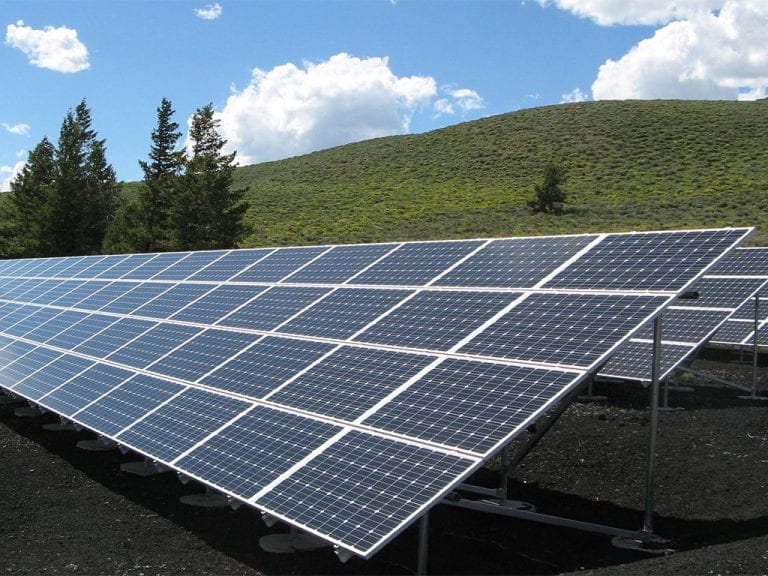
\includegraphics[height=\paperheight]{banner.jpg}}
\usetheme[titlestyle=style1]{trigon}
%\usetheme[sectionstyle=style2]{trigon}

% Define logos to use (comment if no logo)
\biglogo{uliege_faculte_sciencesappliquees_logo_rvb_pos.pdf} % Used on titlepage only
\smalllogo{} % Used on top right corner of regular frames

% ------ If you want to change the theme default colors, do it here ------
%\definecolor{tPrim}{HTML}{00843B}   % Green
%\definecolor{tSec}{HTML}{289B38}    % Green light
%\definecolor{tAccent}{HTML}{F07F3C} % Orange

% ------ Packages and definitions used for this demo. Can be removed ------
\usepackage{appendixnumberbeamer} % To use \appendix command
\pdfstringdefDisableCommands{% Fix hyperref translate warning with \appendix
\def\translate#1{#1}%
}
\usepackage{pgf-pie} % For pie charts
\usepackage{caption} % For subfigures
\usepackage{subcaption} % For subfigures
\usepackage{xspace}
\newcommand{\themename}{\textbf{\textsc{trigon}}\xspace}
\usepackage[scale=2]{ccicons} % Icons for CC-BY-SA
\usepackage{booktabs} % Better tables
\usepackage{amsmath}
\usepackage{amssymb}
\usepackage{amsfonts}
\usepackage{algorithm}
\usepackage{algpseudocodex}
\usepackage{multicol}
\usepackage{booktabs}
\usepackage{colortbl}
\usepackage{listings}
\usepackage{upquote}
\usepackage[scale=0.88]{sourcecodepro}
\usepackage{tikz}
\usepackage{blox}
\usepackage{calc}
\usetikzlibrary{arrows.meta, positioning, calc}




\newcommand{\Z}       {\mathbb{Z} }
\newcommand{\R}       {\mathbb{R} }
\newcommand{\Q}       {\mathbb{Q} }
\newcommand{\N}       {\mathbb{N} }
\newcommand{\spa}     {\text{span}}
\newcommand{\lin}     {\text{span}}
\newcommand{\inter}   {\text{int} }
\newcommand{\st}{\mathrm{s.t.}}
\definecolor{myRed}{RGB}{209,34,57} 

% Modern syntax highlighting palette (GitHub / VS Code style)
\definecolor{codeKw}{RGB}{0, 92, 197}         % Deep royal blue for keywords
\definecolor{codeStr}{RGB}{163, 21, 21}       % Warm crimson for strings
\definecolor{codeComment}{RGB}{106, 115, 125} % Muted slate gray for comments
\definecolor{codeBg}{RGB}{248, 249, 250}      % Soft background card
\definecolor{codeBorder}{RGB}{222, 226, 230}  % Subtle border
\definecolor{codeLineNum}{RGB}{175, 180, 185} % Muted line numbers

\lstset{
    language=Python,
    basicstyle=\linespread{1.05}\ttfamily\footnotesize,
    numbers=left,
    numberstyle=\tiny\color{codeLineNum},
    numbersep=8pt,
    frame=single,
    rulecolor=\color{codeBorder},
    backgroundcolor=\color{codeBg},
    showstringspaces=false,
    tabsize=4,
    keywordstyle=\color{codeKw}\bfseries,
    stringstyle=\color{codeStr},
    commentstyle=\color{codeComment}\itshape,
    columns=flexible,
    keepspaces=true,
    breaklines=true,
    xleftmargin=12pt,
    xrightmargin=4pt
}

%==============================================================================
%                               BEGIN DOCUMENT
%==============================================================================
\begin{document}




%--------------------------------------
% Create title frame
\titleframe

%--------------------------------------
% Table of contents
\begin{frame}{Overview}
  \setbeamertemplate{section in toc}[sections numbered]
  \tableofcontents[hideallsubsections]
\end{frame}

%==============================================================================
\section{Introduction}
%==============================================================================

\begin{frame}{What is a Power Flow Analysis?}
    \textbf{Power flow (or load flow) analysis} determines the steady-state \textit{electrical operating state} of an AC power system under specified generation, consumption, and voltage control conditions.
    
    \begin{columns}
        \begin{column}{0.5\textwidth}
            \textbf{The State Variables to Determine:}
            \begin{itemize}
                \item Voltage magnitude $V_k$ at every bus $k$
                \item Voltage phase angle $\theta_k$ at every bus $k$
            \end{itemize}
            \vspace{0.15cm}
            $$\mathbf{\bar{V}} = \begin{bmatrix} V_1 e^{j\theta_1} & \cdots & V_n e^{j\theta_n} \end{bmatrix}^T$$
        \end{column}
        \begin{column}{0.5\textwidth}
            \textbf{Derived Quantities (from $\mathbf{\bar{V}}$):}
            \begin{itemize}
                \item Branch currents $\bar{I}_{km}$ and loadings
                \item Active/reactive flows $P_{km}, Q_{km}$
                \item Transmission losses $P_{\text{loss}}, Q_{\text{loss}}$
                \item Generator reactive outputs $Q_{Gk}$
            \end{itemize}
        \end{column}
    \end{columns}
    
    \vspace{0.25cm}
    \textbf{The Core Principle:} Once the complex bus voltages $\mathbf{\bar{V}}$ are known, every other physical quantity in the network is directly computed via Ohm's and Kirchhoff's laws.
\end{frame}

\begin{frame}[allowframebreaks]{Why Isn't This Standard Linear Circuit Analysis?}
    \begin{columns}
        \begin{column}{0.5\textwidth}
            \textbf{Linear Circuit Theory:}
            \begin{itemize}
                \item Independent current or voltage sources
                \item Nodal analysis with linear impedances:
                $$\mathbf{\bar{I}} = \mathbf{Y}_{\text{bus}} \mathbf{\bar{V}} \implies \mathbf{\bar{V}} = \mathbf{Y}_{\text{bus}}^{-1} \mathbf{\bar{I}}$$
                \item Solved in a single linear step
            \end{itemize}
        \end{column}
        \begin{column}{0.5\textwidth}
            \textbf{Power System Reality:}
            \begin{itemize}
                \item Loads consume constant \textbf{power} ($P_L, Q_L$), largely independent of voltage
                \item Generators regulate active power $P_G$ and voltage magnitude $V_G$
                \item Injections: $S_k = \bar{V}_k \bar{I}_k^* = \bar{V}_k (\mathbf{Y}_{\text{bus}}\mathbf{\bar{V}})_k^*$
            \end{itemize}
        \end{column}
    \end{columns}

    \begin{block}{The Non-Linearity Challenge}
        The relationship between power injections and bus voltages involves quadratic terms ($V_k^2$) and trigonometric functions of angle differences.
        This forms a system of \textbf{non-linear algebraic equations} that must be solved using iterative numerical algorithms!
    \end{block}
\end{frame}

\begin{frame}{Why Do We Use Power Flow? (Operations \& Reliability)}
    Power flow is the foundational simulation tool for grid operators and utilities:
    
    \begin{itemize}
        \item \textbf{Operational Security \& Real-Time Monitoring}:
        \begin{itemize}
            \item Verify that all transmission line and transformer currents stay within thermal limits ($I_{km} \le I_{\max}$) to prevent line sag or cable damage
            \item Ensure bus voltages remain strictly within regulatory safety bounds ($0.95 \le V_k \le 1.05\text{ pu}$) to prevent equipment tripping
        \end{itemize}
        \vspace{0.2cm}
        \item \textbf{Contingency Analysis ($N-1$ Security Criterion)}:
        \begin{itemize}
            \item Power systems are legally required to withstand the sudden tripping of any single asset (line, transformer, generator) without causing cascading overloads
            \item TSOs (e.g. Elia, RTE, TenneT) run thousands of automated power flows every hour to screen for $N-1$ vulnerabilities
        \end{itemize}
    \end{itemize}
\end{frame}

\begin{frame}{Why Do We Use Power Flow? (Planning, Markets \& Stability)}
    \begin{itemize}
        \item \textbf{Grid Expansion \& Long-Term Planning}:
        \begin{itemize}
            \item Forecast where bottlenecks will appear 5--20 years ahead
            \item Size and place new transmission lines, subsea cables, transformers, or reactive compensation devices (STATCOM, synchronous condensers)
        \end{itemize}
        \vspace{0.15cm}
        \item \textbf{Renewables Integration \& Electricity Markets}:
        \begin{itemize}
            \item Calculate grid hosting capacity for massive offshore wind and utility-scale solar
            \item Verify the physical feasibility of market clearing schedules and compute Locational Marginal Prices (LMP) and transmission congestion charges
        \end{itemize}
        \vspace{0.15cm}
        \item \textbf{Foundation for Dynamic Stability Studies}:
        \begin{itemize}
            \item Power flow provides the initial equilibrium point $(\mathbf{V}_0, \boldsymbol{\theta}_0)$ required to initialize transient stability, small-signal stability, and voltage stability simulations
        \end{itemize}
    \end{itemize}
\end{frame}

\begin{frame}[allowframebreaks]{Power Flow Problem Statement \& Bus Types}
    At every bus $k$, four physical quantities describe the state:
    $$(V_k, \theta_k, P_k, Q_k)$$
    In power flow analysis, \textbf{two variables are specified} (boundary conditions) and \textbf{two variables are unknown}:
    
    \begin{itemize}
        \item \textbf{PQ Buses (Load buses)}:
        \begin{itemize}
            \item Active power $P_k^{\text{spec}}$ and reactive power $Q_k^{\text{spec}}$ are specified (consumed by loads, or injected by non-voltage-regulating renewable generators).
            \item \textbf{Unknowns to find:} Voltage magnitude $V_k$ and phase angle $\theta_k$.
        \end{itemize} \newpage
        \item \textbf{PV Buses (Voltage-regulated generator buses)}:
        \begin{itemize}
            \item Active power $P_k^{\text{spec}}$ and voltage magnitude $V_k^{\text{spec}}$ are specified (controlled via governor and Automatic Voltage Regulator (AVR)).
            \item \textbf{Unknowns to find:} Phase angle $\theta_k$ and reactive power $Q_k$.
            \item \textit{Reactive limits:} If $Q_k$ hits a capability limit ($Q_{\min}$ or $Q_{\max}$), the generator cannot maintain voltage; the bus switches to a \textbf{PQ bus} with $Q_k = Q_{\text{limit}}$.
        \end{itemize}
        \item \textbf{One Slack Bus (Swing or Reference bus)}:
        \begin{itemize}
            \item Sets the angular reference for the entire system: $\theta_{\text{slack}} = 0^\circ$.
            \item Voltage magnitude is specified (typically $V_{\text{slack}} = 1.0\text{ pu}$).
            \item \textbf{Unknowns to find:} Active power $P_{\text{slack}}$ and reactive power $Q_{\text{slack}}$.
        \end{itemize}
    \end{itemize}
    
    \begin{alertblock}{Why is a Slack Bus strictly necessary?}
        Transmission losses ($P_{\text{loss}} = \sum R_{km} I_{km}^2$) depend on the branch currents, which are unknown before voltages are found!
        Therefore, total generation cannot be fixed in advance:
        $$\sum P_{G} = \sum P_{L} + P_{\text{loss}}(\mathbf{\bar{V}})$$
        The slack bus generator automatically acts as the buffer that balances the remaining active and reactive power of the grid.
    \end{alertblock}
\end{frame}

\begin{frame}[allowframebreaks]{A First Tiny Example (3-Bus System)}
    \begin{center}
        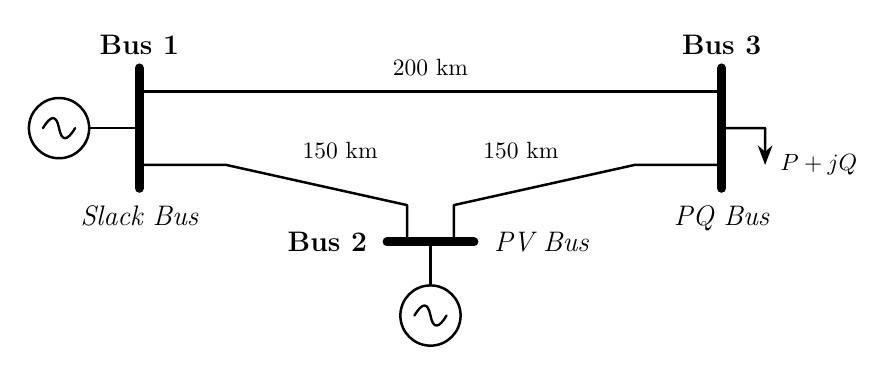
\begin{tikzpicture}[scale=0.85, every node/.style={transform shape}, >=Stealth, line cap=round, line join=round]
    % Styles
    \tikzset{
        busbar/.style={line width=3.2pt, black},
        transmission/.style={line width=0.9pt, black},
        element/.style={line width=0.9pt, black}
    }
    
    % Geometry coordinates (origin at center between Bus 1 and Bus 3, at bottom-line level y=0)
    
    % --- Bus 1 ---
    \coordinate (B1_top) at (-4.35, 1.45);
    \coordinate (B1_bot) at (-4.35, -0.35);
    \coordinate (B1_conn_top) at (-4.35, 1.10);
    \coordinate (B1_conn_mid) at (-4.35, 0.55);
    \coordinate (B1_conn_bot) at (-4.35, 0.0);
    
    \draw[busbar] (B1_bot) -- (B1_top);
    \node[above=2pt, font=\large\bfseries] at (B1_top) {Bus 1};
    \node[below=4pt, font=\large\itshape] at (B1_bot) {Slack Bus};
    
    % --- Bus 3 ---
    \coordinate (B3_top) at (4.35, 1.45);
    \coordinate (B3_bot) at (4.35, -0.35);
    \coordinate (B3_conn_top) at (4.35, 1.10);
    \coordinate (B3_conn_mid) at (4.35, 0.55);
    \coordinate (B3_conn_bot) at (4.35, 0.0);
    
    \draw[busbar] (B3_bot) -- (B3_top);
    \node[above=2pt, font=\large\bfseries] at (B3_top) {Bus 3};
    \node[below=4pt, font=\large\itshape] at (B3_bot) {PQ Bus};
    
    % --- Bus 2 ---
    \coordinate (B2_left) at (-0.65, -1.15);
    \coordinate (B2_right) at (0.65, -1.15);
    \coordinate (B2_conn_left) at (-0.35, -1.15);
    \coordinate (B2_conn_mid) at (0.0, -1.15);
    \coordinate (B2_conn_right) at (0.35, -1.15);
    
    \draw[busbar] (B2_left) -- (B2_right);
    \node[left=5pt, font=\large\bfseries] at (B2_left) {Bus 2};
    \node[right=5pt, font=\large\itshape] at (B2_right) {PV Bus};
    
    % --- Transmission Lines ---
    % Line 1-3 (Top line)
    \draw[transmission] (B1_conn_top) -- (B3_conn_top)
        node[midway, above=3pt, font=\normalsize] {200 km};
    
    % Line 1-2
    \draw[transmission] (B1_conn_bot) -- (-3.05, 0.0) -- (-0.35, -0.60) -- (B2_conn_left);
    \node[font=\normalsize] at (-1.35, 0.22) {150 km};
    
    % Line 2-3
    \draw[transmission] (B2_conn_right) -- (0.35, -0.60) -- (3.05, 0.0) -- (B3_conn_bot);
    \node[font=\normalsize] at (1.35, 0.22) {150 km};
    
    % --- Generator at Bus 1 ---
    \coordinate (G1_center) at (-5.55, 0.55);
    \draw[element] (B1_conn_mid) -- ($(G1_center) + (0.45, 0)$);
    \draw[element] (G1_center) circle (0.45);
    % Sine wave inside G1
    \draw[element, line width=0.85pt] 
        ($(G1_center) + (-0.24, 0)$) 
        .. controls ($(G1_center) + (-0.12, 0.20)$) and ($(G1_center) + (-0.04, 0.20)$) .. (G1_center)
        .. controls ($(G1_center) + (0.04, -0.20)$) and ($(G1_center) + (0.12, -0.20)$) .. ($(G1_center) + (0.24, 0)$);
        
    % --- Generator at Bus 2 ---
    \coordinate (G2_center) at (0.0, -2.25);
    \draw[element] (B2_conn_mid) -- ($(G2_center) + (0, 0.45)$);
    \draw[element] (G2_center) circle (0.45);
    % Sine wave inside G2
    \draw[element, line width=0.85pt] 
        ($(G2_center) + (-0.24, 0)$) 
        .. controls ($(G2_center) + (-0.12, 0.20)$) and ($(G2_center) + (-0.04, 0.20)$) .. (G2_center)
        .. controls ($(G2_center) + (0.04, -0.20)$) and ($(G2_center) + (0.12, -0.20)$) .. ($(G2_center) + (0.24, 0)$);
        
    % --- Load at Bus 3 ---
    \coordinate (L3_turn) at ($(B3_conn_mid) + (0.65, 0)$);
    \coordinate (L3_arrow) at ($(L3_turn) + (0, -0.55)$);
    \draw[element] (B3_conn_mid) -- (L3_turn);
    \draw[element, ->, >=Stealth] (L3_turn) -- (L3_arrow);
    \node[right=3pt, font=\normalsize] at (L3_arrow) {$P + jQ$};

\end{tikzpicture}

    \end{center}
    
    \begin{columns}
        \begin{column}{0.5\linewidth}
            \textbf{Buses:}
            \begin{itemize}
                \item \textbf{Bus 1 (Slack):} $V_1 = 1.00\text{ pu}, \theta_1 = 0^\circ$
                \item \textbf{Bus 2 (PV):} $V_2 = 1.05\text{ pu}$, generating $P_2 = 2.0\text{ pu}$ ($200\text{ MW}$)
                \item \textbf{Bus 3 (PQ):} Load consuming $P_3 = 5.0\text{ pu}$ ($500\text{ MW}$) and $Q_3 = 1.0\text{ pu}$ ($100\text{ Mvar}$)
            \end{itemize}
        \end{column}
        \begin{column}{0.5\linewidth}
            \textbf{Lines (Base: $345\text{ kV}$, $100\text{ MVA}$):}
            \begin{itemize}
                \item $X = 0.376\ \Omega/\text{km}$, $R = 0.037\ \Omega/\text{km}$
                \item Lengths: $L_{12} = 150\text{ km}$, $L_{23} = 150\text{ km}$, $L_{31} = 200\text{ km}$
                \item Base impedance: $Z_B = 345^2 / 100 = 1190.25\ \Omega$
                \item Current rating: $I_{\max} = 0.20\text{ kA}$
            \end{itemize}
        \end{column}
    \end{columns}
\end{frame}

\begin{frame}{Modeling the System in PandaPower}
    We will see how to formulate mathematically the problem and solve it from scratch.
    
    Usually, engineers use specialized power system software. One such open-source, Python-based tool is \textbf{PandaPower} \cite{thurner2018pandapower}.

    \begin{center}
        \vspace{0.4cm}
        \href{https://colab.research.google.com/drive/103VIzly2huoS-PjnYdbCaeBS1dunJS7H?usp=sharing}{\beamergotobutton{Open PandaPower 3-Bus Model in Google Colab}}
    \end{center}
\end{frame}

\begin{frame}[fragile, allowframebreaks]
    \frametitle{Creation of the Power Flow Model with PandaPower}
    \lstinputlisting{pandapower_net.py}
\end{frame}

\begin{frame}{Results of the 3-Bus Example: Bus State}

    

    \begin{columns}
        \begin{column}{0.6\textwidth}
                \begin{table}[h]
        \centering
        \footnotesize
        \setlength{\tabcolsep}{6pt}
        \begin{tabular}{llcccc}
            \toprule
            \textbf{Bus} & \textbf{Type} & $\mathbf{V}$ \textbf{[pu]} & $\boldsymbol{\theta}$ \textbf{[$^\circ$]} & $\mathbf{P}$ \textbf{[MW]} & $\mathbf{Q}$ \textbf{[Mvar]} \\
            \midrule
            Bus 1 & Slack & 1.000 & 0.00 & \color{blue}\textbf{-308.38} & \color{blue}\textbf{+81.61} \\
            Bus 2 & PV    & 1.050 & \color{blue}\textbf{-2.07} & -200.00 & \color{blue}\textbf{-266.74} \\
            Bus 3 & PQ    & \color{blue}\textbf{0.978} & \color{blue}\textbf{-8.79} & +500.00 & +100.00 \\
            \bottomrule
        \end{tabular}
    \end{table}
            \textbf{Legend \& Conventions:}
            \begin{itemize}
                \item Standard text: \textbf{Specified input data}
                \item \color{blue}\textbf{Bold blue text: Computed by power flow}
                \item Sign convention (PandaPower net flow):
                \begin{itemize}
                    \item Negative $(-)$: Net injection (generation)
                    \item Positive $(+)$: Net withdrawal (load)
                \end{itemize}
            \end{itemize}
        \end{column}
        \begin{column}{0.35\textwidth}
            \textbf{Physical Observations:}
            \begin{itemize}
                \item Bus 1 generator supplies $308.38\text{ MW}$ to balance total load plus line losses
                \item Bus 2 generator injects $266.74\text{ Mvar}$ to hold voltage at $1.05\text{ pu}$
                \item Voltage at load Bus 3 drops to $0.978\text{ pu}$ ($\Delta \theta = -8.79^\circ$)
            \end{itemize}
        \end{column}
    \end{columns}
\end{frame}

\begin{frame}{Results of the 3-Bus Example: Line Flows \& Loading}
    \begin{table}[h]
        \centering
        \scriptsize
        \setlength{\tabcolsep}{4pt}
        \begin{tabular}{lcccccccc}
            \toprule
            \textbf{Line} & \textbf{From $\to$ To} & $\mathbf{P_{\text{from}}}$ & $\mathbf{P_{\text{to}}}$ & $\mathbf{P_{\text{loss}}}$ & $\mathbf{Q_{\text{loss}}}$ & $\mathbf{I}$ & $\mathbf{I_{\max}}$ & \textbf{Loading} \\
            & & [MW] & [MW] & [MW] & [Mvar] & [kA] & [kA] & [\%] \\
            \midrule
            Line 1 & Bus 1 $\to$ Bus 2 & +69.0 & -68.2 & 0.80 & 8.08 & 0.22 & 0.20 & \color{orange!90!black}\textbf{109.8\,\%} \\
            Line 2 & Bus 2 $\to$ Bus 3 & +268.2 & -264.2 & 3.97 & 40.30 & 0.49 & 0.20 & \color{red}\textbf{245.2\,\%} \\
            Line 3 & Bus 3 $\to$ Bus 1 & -235.8 & +239.4 & 3.62 & 36.75 & 0.40 & 0.20 & \color{red}\textbf{201.2\,\%} \\
            \midrule
            \multicolumn{2}{l}{\textbf{Total Losses}} & & & \textbf{8.39} & \textbf{85.13} & & & \\
            \bottomrule
        \end{tabular}
    \end{table}

    \vspace{0.1cm}
    \begin{columns}
        \begin{column}{0.5\textwidth}
            \scriptsize
            \textbf{Active Power Balance:}
            \begin{itemize}
                \item Total Gen: $P_G = 308.38 + 200.00 = 508.38\text{ MW}$
                \item Total Load: $P_L = 500.00\text{ MW}$
                \item \textbf{Losses:} $P_G - P_L = \mathbf{8.38\text{ MW}}$ ($1.65\%$ of load)
                \item Matches sum of line losses: $8.39\text{ MW}$
            \end{itemize}
        \end{column}
        \begin{column}{0.5\textwidth}
            \scriptsize
            \textbf{Engineering Diagnosis:}
            \begin{itemize}
                \item Bus voltages are healthy ($0.978 - 1.05\text{ pu}$)
                \item \alert{\textbf{Lines 2 and 3 are severely overloaded}} ($245\%$ and $201\%$)!
                \item Protection relays would trip these lines, risking cascading failure without re-dispatch!
            \end{itemize}
        \end{column}
    \end{columns}
\end{frame}

%==============================================================================
\section{The power flow equations}
%==============================================================================

\begin{frame}[allowframebreaks]{The Nodal Admittance Matrix $\mathbf{Y}_{\text{bus}}$}
    Consider a power system with bus set $\mathcal{N} = \{1, \dots, n\}$ interconnected by transmission lines modeled by equivalent $\pi$ circuits:
    
    \begin{itemize}
        \item For line connecting buses $k$ and $m$: series impedance $\bar{z}_{km} = r_{km} + j x_{km}$, series admittance $\bar{y}_{km} = 1/\bar{z}_{km}$ (and $\bar{y}_{km} = 0$ if no line exists)
        \item Line total charging shunt susceptance $b_{km}^{\text{sh}}$, split equally as $j \omega C_{km}/2$ at each terminal
        \item Shunt element connected at node $k$ (e.g. reactor/capacitor): $Y_{k,sh} = G_{k,sh} + j B_{k,sh}$
        \item Total shunt admittance between bus $k$ and ground:
        $$\mathcolor[RGB]{00,99,00}{Y_{kG}} = Y_{k,sh} + \sum_{m \in \mathcal{N}_k} j \frac{\omega C_{km}}{2}$$
    \end{itemize}

    
    \begin{figure}[htbp]
        \centering
        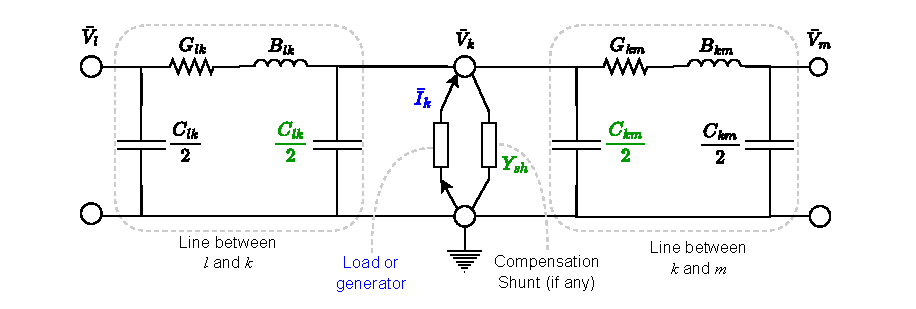
\includegraphics[width=0.95\textwidth]{images/bus_injection_model.pdf}
        \caption{Current injection at bus $k$ as a function of branch flows to neighbors ($l, m$) and shunt elements to ground.}
        \label{fig:bus_injection}
    \end{figure}

    By Kirchhoff's Current Law (KCL), the net current injection $\mathcolor{blue}{\bar{I}_k}$ into bus $k$ is:
    \begin{equation}
        \mathcolor{blue}{\bar{I}_k} = \mathcolor[RGB]{00,99,00}{Y_{kG}} \bar{V}_k + \sum_{m \in \mathcal{N} \setminus \{k\}} \bar{y}_{km} (\bar{V}_k - \bar{V}_m) \label{eq:bus_inj}
    \end{equation}

    Factoring out the bus voltages:
    \begin{equation}
        \mathcolor{blue}{\bar{I}_k} = \underbrace{\left(\mathcolor[RGB]{00,99,00}{Y_{kG}} + \sum_{m \in \mathcal{N} \setminus \{k\}} \bar{y}_{km} \right)}_{Y_{kk}} \bar{V}_k + \sum_{m \in \mathcal{N} \setminus \{k\}} \underbrace{(-\bar{y}_{km})}_{Y_{km}} \bar{V}_m
    \end{equation}
    
    In matrix form for all $n$ buses:
    \begin{equation}
        \mathbf{\bar{I}} = \mathbf{Y}_{\text{bus}} \mathbf{\bar{V}} \label{eq:bus_inj_mat}
    \end{equation}

    \begin{block}{Rules for building $\mathbf{Y}_{\text{bus}}$ by inspection:}
        \begin{itemize}
            \item \textbf{Diagonal element $Y_{kk}$:} sum of all admittances connected to bus $k$ (series lines + shunts)
            \item \textbf{Off-diagonal element $Y_{km}$ ($m \neq k$):} negative of the series admittance connecting bus $k$ and bus $m$ (hence $Y_{km} = Y_{mk}$ for bilateral lines)
        \end{itemize}
    \end{block}
    \end{frame}

\begin{frame}[allowframebreaks]{Power Flow Equations in Polar Coordinates}
    In power systems, boundary conditions are given in powers rather than currents.
    The complex power injection vector is:
    \begin{equation}
        \mathbf{S} = \mathbf{P} + j \mathbf{Q} = \mathrm{diag}(\mathbf{\bar{V}}) \mathbf{\bar{I}}^{\star} = \mathbf{\bar{V}} \circ (\mathbf{Y}_{\text{bus}} \mathbf{\bar{V}})^{\star} \label{eq:pf}
    \end{equation}
    where $\circ$ denotes the Hadamard (element-wise) product.
    
    For a single bus $k$:
    \begin{equation}
        S_k = P_k + j Q_k = \bar{V}_k \bar{I}_k^{\star} = \bar{V}_k \sum_{m=1}^n Y_{km}^{\star} \bar{V}_m^{\star}
    \end{equation}

    \newpage
    Expressing voltages in polar coordinates and admittance in rectangular coordinates:
    $$\bar{V}_k = V_k e^{j\theta_k}, \quad \bar{V}_m = V_m e^{j\theta_m}, \quad Y_{km} = G_{km} + j B_{km}$$
    
    Then:
    $$S_k = \sum_{m=1}^n V_k V_m e^{j(\theta_k - \theta_m)} (G_{km} - j B_{km})$$
    
    Using Euler's identity $e^{j\theta_{km}} = \cos\theta_{km} + j \sin\theta_{km}$ with phase difference $\theta_{km} = \theta_k - \theta_m$:
    \begin{align}
        P_k &= \underbrace{V_k \sum_{m=1}^n V_m (G_{km} \cos\theta_{km} + B_{km} \sin\theta_{km})}_{\mathcolor[RGB]{00,99,00}{p_k(\mathbf{V}, \boldsymbol{\theta})}}\label{eq:pf_P} \\[0.5em]
        Q_k &= \underbrace{V_k \sum_{m=1}^n V_m (G_{km} \sin\theta_{km} - B_{km} \cos\theta_{km})}_{\mathcolor[RGB]{00,99,00}{q_k(\mathbf{V}, \boldsymbol{\theta})}}\label{eq:pf_Q}
    \end{align}

    \newpage
    Separating the self-term ($m=k$, where $\theta_{kk}=0, \cos 0 = 1, \sin 0 = 0$):
    \begin{align}
        P_k &= G_{kk} V_k^2 + V_k \sum_{m \neq k} V_m (G_{km} \cos\theta_{km} + B_{km} \sin\theta_{km}) \\[0.5em]
        Q_k &= -B_{kk} V_k^2 + V_k \sum_{m \neq k} V_m (G_{km} \sin\theta_{km} - B_{km} \cos\theta_{km})
    \end{align}
    
    \begin{itemize}
        \item $G_{kk} V_k^2$ represents local active power dissipation
        \item $-B_{kk} V_k^2$ represents local reactive power injected by shunt susceptance
        \item The summation over $m \neq k$ represents the active/reactive power exchanged with neighboring buses
    \end{itemize}
\end{frame}

\begin{frame}[allowframebreaks]{Number of Equations and Unknowns}
    In an $n$-bus power system with $n_{PQ}$ PQ buses, $n_{PV}$ PV buses, and 1 slack bus ($n = n_{PQ} + n_{PV} + 1$):
    
    \begin{table}[h]
        \centering
        \small
        \begin{tabular}{lcccc}
            \toprule
            \textbf{Bus Type} & \textbf{Count} & \textbf{Specified Knowns} & \textbf{Iterative Unknowns} & \textbf{Equations Used} \\
            \midrule
            PQ Bus    & $n_{PQ}$ & $P_k^{\text{spec}}, Q_k^{\text{spec}}$ & $V_k, \theta_k$ & $P_k - p_k = 0, \ Q_k - q_k = 0$ \\
            PV Bus    & $n_{PV}$ & $P_k^{\text{spec}}, V_k^{\text{spec}}$ & $\theta_k$      & $P_k - p_k = 0$ \\
            Slack Bus & 1        & $V_s^{\text{spec}}, \theta_s^{\text{spec}} = 0$ & none (in NR)    & none (in NR) \\
            \midrule
            \textbf{Total} & $n$ & $2n$ knowns & $\mathbf{2n_{PQ} + n_{PV}}$ & $\mathbf{2n_{PQ} + n_{PV}}$ equations \\
            \bottomrule
        \end{tabular}
    \end{table}

    \newpage
    \textbf{Post-processing quantities (computed after convergence):}
    \begin{itemize}
        \item Slack bus power injections: $P_{\text{slack}} = p_{\text{slack}}(\mathbf{V}, \boldsymbol{\theta})$ and $Q_{\text{slack}} = q_{\text{slack}}(\mathbf{V}, \boldsymbol{\theta})$
        \item Generator reactive power at PV buses: $Q_k = q_k(\mathbf{V}, \boldsymbol{\theta})$ for $k \in \mathcal{N}_{PV}$
        \item Branch currents, active/reactive line flows, and system losses
    \end{itemize}
\end{frame}

%==============================================================================
\section{Power flow solution method}
%==============================================================================

\begin{frame}[allowframebreaks]{Power Flow Solution via Newton-Raphson}
    Let the specified (known) active and reactive powers be $\mathcolor{blue}{P_k^0}$ and $\mathcolor{blue}{Q_k^0}$. \\
    We define the \textbf{power mismatch functions}:
    \begin{align*}
        \Delta P_k(\mathbf{V}, \boldsymbol{\theta}) &= \mathcolor{blue}{P_k^0} \mathcolor[RGB]{00,99,00}{- p_k(\mathbf{V}, \boldsymbol{\theta})}, \quad \forall k \in \mathcal{N}_{PQ} \cup \mathcal{N}_{PV} \\
        \Delta Q_k(\mathbf{V}, \boldsymbol{\theta}) &= \mathcolor{blue}{Q_k^0} \mathcolor[RGB]{00,99,00}{- q_k(\mathbf{V}, \boldsymbol{\theta})}, \quad \forall k \in \mathcal{N}_{PQ}
    \end{align*}

    We want to find a solution such that $$\Delta P_k(\mathbf{V}, \boldsymbol{\theta}) = \Delta Q_k(\mathbf{V}, \boldsymbol{\theta}) = 0,$$
    i.e. we want to find values for unknown variables to explain the known variables.
    
    This forms a set of $2 n_{PQ} + n_{PV}$ non-linear algebraic equations in $2 n_{PQ} + n_{PV}$ unknown state variables:
    $$\mathbf{x} = \begin{bmatrix} \boldsymbol{\theta}_{PQ, PV} \\ \mathbf{V}_{PQ} \end{bmatrix}, \qquad \mathbf{F}(\mathbf{x}) = \begin{bmatrix} \Delta \mathbf{P}(\mathbf{x}) \\ \Delta \mathbf{Q}(\mathbf{x}) \end{bmatrix} = \mathbf{0}$$
    
    The standard method to solve this non-linear system is the \textbf{Newton-Raphson method}.
\end{frame}

\begin{frame}{Newton-Raphson Method in 1D: Principles}
    Suppose we want to find $x$ such that the mismatch $g(x) = c - f(x) = 0$.
    
    \begin{itemize}
        \item Start with an initial guess $x^{(0)}$ at iteration $i=0$
        \item First-order Taylor approximation around $x^{(i)}$:
        $$g(x^{(i)} + \Delta x) \approx g(x^{(i)}) + g'(x^{(i)}) \Delta x = 0$$
        \item Solve for the update step: $\Delta x = -\dfrac{g(x^{(i)})}{g'(x^{(i)})} = \dfrac{c - f(x^{(i)})}{f'(x^{(i)})}$
        \item Update iterate: $x^{(i+1)} = x^{(i)} + \Delta x$ and repeat until $|g(x^{(i)})| \le \epsilon$
    \end{itemize}
    
    \vspace{0.15cm}
    \alert{\textbf{Quadratic Convergence:}} If $x^{(0)}$ is near the root, $|x^{(i+1)} - x^*| \le K |x^{(i)} - x^*|^2$.
    The number of accurate decimal digits roughly doubles at each iteration!
\end{frame}

\begin{frame}{Newton-Raphson 1D: Step-by-Step Convergence}

    
    \begin{columns}
        \begin{column}{0.48\textwidth}
            \footnotesize
            \textbf{Example: Solve $g(x) = 4 - x^3 = 0$}
            \vspace{-0.15cm}
            $$\Delta x^{(i)} = \frac{4 - (x^{(i)})^3}{3 (x^{(i)})^2}, \quad x^{(i+1)} = x^{(i)} + \Delta x^{(i)}$$
            
            \vspace{-0.1cm}
            \scriptsize
            \begin{tabular}{ccccc}
                \toprule
                $i$ & $x^{(i)}$ & $g(x^{(i)})$ & $\Delta x^{(i)}$ & $|x^{(i)}-x^*|$ \\
                \midrule
                \alt<1>{\color{red}\bfseries 0 & \color{red}\bfseries 3.5000 & \color{red}\bfseries -38.88 & \color{red}\bfseries -1.058 & \color{red}\bfseries 1.913}{0 & 3.5000 & -38.88 & -1.058 & 1.913} \\
                \alt<2>{\color{orange!90!black}\bfseries 1 & \color{orange!90!black}\bfseries 2.4422 & \color{orange!90!black}\bfseries -10.57 & \color{orange!90!black}\bfseries -0.590 & \color{orange!90!black}\bfseries 0.855}{1 & 2.4422 & -10.57 & -0.590 & 0.855} \\
                \alt<3>{\color{purple}\bfseries 2 & \color{purple}\bfseries 1.8517 & \color{purple}\bfseries -2.35 & \color{purple}\bfseries -0.228 & \color{purple}\bfseries 0.264}{2 & 1.8517 & -2.35 & -0.228 & 0.264} \\
                \alt<4>{\color{green!60!black}\bfseries 3 & \color{green!60!black}\bfseries 1.6233 & \color{green!60!black}\bfseries -0.27 & \color{green!60!black}\bfseries -0.035 & \color{green!60!black}\bfseries 0.036}{3 & 1.6233 & -0.27 & -0.035 & 0.036} \\
                \bottomrule
            \end{tabular}

            \vspace{0.25cm}
            \href{https://colab.research.google.com/drive/12tCcO6kPxkoScAGnUYxgumS3CVSBSmtJ?usp=sharing}{\beamergotobutton{Python Colab Implementation}}
            \quad
            \href{https://github.com/bcornelusse/ELEC0447-analysis-power-systems/blob/master/Lectures/IntroPowerFlow/interactive_nr_visualizer.html}{\beamergotobutton{Interactive Web Visualizer}}
        \end{column} \hfill
        \begin{column}{0.48\textwidth}
            \centering
            \begin{tikzpicture}[xscale=1.25, yscale=0.07]
                % Axes
                \draw[->, >=stealth, thick] (0.8,0) -- (4.0,0) node[right] {\footnotesize $x$};
                \draw[->, >=stealth, thick] (1.0,-42) -- (1.0,8) node[above, blue] {\footnotesize $g(x) = 4 - x^3$};
                \draw[dashed, gray!60] (0.8,0) -- (4.0,0);
                
                % Function curve
                \draw[domain=1.0:3.8, smooth, variable=\x, blue, very thick] plot ({\x}, {4 - \x*\x*\x});
                %\node[blue, right] at (1.1, 5) {\footnotesize $g(x) = 4 - x^3 = 0$};
                \node[green!60!black, below] at (1.587, 0) {\tiny $x^* \approx 1.587$};
                \fill[green!60!black] (1.587, 0) circle (1.5pt);

                % Step 0
                \only<1->{
                    \draw[dotted, thick, red] (3.5, 0) -- (3.5, -38.875);
                    \fill[red] (3.5, -38.875) circle (1.5pt);
                    \fill[red] (3.5, 0) circle (1.5pt) node[above, red] {\scriptsize $x^{(0)}=3.5$};
                }
                
                % Step 1
                \only<2->{
                    \draw[thick, orange!90!black, -{Stealth[length=2mm]}] (3.5, -38.875) -- (2.442, 0);
                    \draw[dotted, thick, red] (2.442, 0) -- (2.442, -10.566);
                    \fill[red] (2.442, -10.566) circle (1.5pt);
                    \fill[orange!90!black] (2.442, 0) circle (1.5pt) node[above] {\scriptsize $x^{(1)}$};
                }

                % Step 2
                \only<3->{
                    \draw[thick, purple, -{Stealth[length=2mm]}] (2.442, -10.566) -- (1.852, 0);
                    \draw[dotted, thick, red] (1.852, 0) -- (1.852, -2.349);
                    \fill[red] (1.852, -2.349) circle (1.5pt);
                    \fill[purple] (1.852, 0) circle (1.5pt) node[above] {\scriptsize $x^{(2)}$};
                }

                % Step 3
                \only<4->{
                    \draw[thick, green!60!black, -{Stealth[length=2mm]}] (1.852, -2.349) -- (1.623, 0);
                    \fill[green!60!black] (1.623, 0) circle (1.5pt) node[above left] {\scriptsize $x^{(3)}$};
                }
            \end{tikzpicture}
        \end{column}
    \end{columns}
\end{frame}

\begin{frame}[allowframebreaks]{Newton-Raphson for Power Flow}
    We apply the same principle in dimension $M = 2 n_{PQ} + n_{PV}$.
    At iteration $(i)$, the linearized mismatch system is:
    \begin{equation}
        \mathbf{J}(\mathbf{x}^{(i)}) \Delta \mathbf{x}^{(i)} = \mathbf{F}(\mathbf{x}^{(i)})
    \end{equation}
    
    where the \textbf{Jacobian matrix} $\mathbf{J}$ contains the partial derivatives:
    \begin{equation}
        \begin{bmatrix}
            \mathbf{J}_{P\theta} & \mathbf{J}_{PV} \\[0.6em]
            \mathbf{J}_{Q\theta} & \mathbf{J}_{QV}
        \end{bmatrix}^{(i)}
        \begin{bmatrix}
            \Delta \boldsymbol{\theta} \\[0.6em]
            \Delta \mathbf{V}
        \end{bmatrix}^{(i)}
        =
        \begin{bmatrix}
            \mathbf{P}^0 - \mathbf{p}(\mathbf{V}^{(i)}, \boldsymbol{\theta}^{(i)}) \\[0.6em]
            \mathbf{Q}^0 - q(\mathbf{V}^{(i)}, \boldsymbol{\theta}^{(i)})
        \end{bmatrix}
    \end{equation}

    \newpage
    The four sub-matrices of the Jacobian are:
    \begin{itemize}
        \item $\mathbf{J}_{P\theta} = \dfrac{\partial \mathbf{P}}{\partial \boldsymbol{\theta}}$ of size $(n_{PQ} + n_{PV}) \times (n_{PQ} + n_{PV})$
        \item $\mathbf{J}_{PV} = \dfrac{\partial \mathbf{P}}{\partial \mathbf{V}}$ of size $(n_{PQ} + n_{PV}) \times n_{PQ}$
        \item $\mathbf{J}_{Q\theta} = \dfrac{\partial \mathbf{Q}}{\partial \boldsymbol{\theta}}$ of size $n_{PQ} \times (n_{PQ} + n_{PV})$
        \item $\mathbf{J}_{QV} = \dfrac{\partial \mathbf{Q}}{\partial \mathbf{V}}$ of size $n_{PQ} \times n_{PQ}$
    \end{itemize}

    \vspace{0.2cm}
    Once $\Delta \boldsymbol{\theta}$ and $\Delta \mathbf{V}$ are calculated by solving the linear system:
    $$\boldsymbol{\theta}^{(i+1)} = \boldsymbol{\theta}^{(i)} + \Delta \boldsymbol{\theta}, \qquad \mathbf{V}^{(i+1)} = \mathbf{V}^{(i)} + \Delta \mathbf{V}$$
\end{frame}

\begin{frame}{Remarks on Practical Implementation}
    \begin{itemize}
        \item \textbf{Avoid Inversion}: We never compute the matrix inverse $\mathbf{J}^{-1}$; instead, we solve the linear system $\mathbf{J} \Delta \mathbf{x} = \Delta \mathbf{F}$ via LU factorization and forward/backward substitution
        \item \textbf{Sparsity Exploitation}: In real power systems, each bus is typically connected to only 2--5 neighboring lines. The Jacobian is extremely sparse (often $>99\%$ zeros). Using sparse matrix algorithms reduces computational cost from $\mathcal{O}(n^3)$ to nearly $\mathcal{O}(n^{1.2})$!
        \item \textbf{Flat Start}: Without prior knowledge, iterations are initialized at a \textit{flat start}:
        $$V_k^{(0)} = 1.0\text{ pu}, \quad \theta_k^{(0)} = 0^\circ \quad \forall k$$
        \item \textbf{Jacobian Reuse}: In modified Newton methods, the Jacobian can be held constant across multiple iterations close to convergence to save computation
    \end{itemize}
\end{frame}

\begin{frame}[allowframebreaks]{Illustration on the 3-Bus Example}
    Let us apply the Newton-Raphson algorithm step-by-step to our 3-bus network:
    \begin{itemize}
        \item Bus 1 is Slack ($V_1 = 1.0\text{ pu}, \theta_1 = 0^\circ$)
        \item Bus 2 is PV ($V_2 = 1.05\text{ pu}, P_2 = -2.0\text{ pu}$) $\to$ unknown: $\theta_2$
        \item Bus 3 is PQ ($P_3 = 5.0\text{ pu}, Q_3 = 1.0\text{ pu}$) $\to$ unknowns: $\theta_3, V_3$
    \end{itemize}
    
    The unknown vector has dimension 3:
    $$\mathbf{x} = \begin{bmatrix} \theta_2 & \theta_3 & V_3 \end{bmatrix}^T$$
    
    \newpage
    \textbf{Step 0: Flat Start Initialization}
    $$\mathbf{x}^{(0)} = \begin{bmatrix} \theta_2^{(0)} & \theta_3^{(0)} & V_3^{(0)} \end{bmatrix}^T = \begin{bmatrix} 0\text{ rad} & 0\text{ rad} & 1.0\text{ pu} \end{bmatrix}^T$$
    
    \textbf{Step 1: Initial Power Mismatches}
    Evaluating $p_2, p_3, q_3$ at $\mathbf{x}^{(0)}$:
    $$\begin{bmatrix}
        \Delta P_2 \\ \Delta P_3 \\ \Delta Q_3
    \end{bmatrix}^{(0)} = 
    \begin{bmatrix}
        P_2^0 - p_2(\mathbf{x}^{(0)}) \\
        P_3^0 - p_3(\mathbf{x}^{(0)}) \\
        Q_3^0 - q_3(\mathbf{x}^{(0)})
    \end{bmatrix} =
    \begin{bmatrix}
        -1.784 \\ +4.897 \\ -0.045
    \end{bmatrix}\text{ pu}$$
    
    \newpage
    \textbf{Step 2: Linear System Solution}
    Compute the $3 \times 3$ Jacobian at $\mathbf{x}^{(0)}$ and solve:
    $$\begin{bmatrix}
        \dfrac{\partial p_2}{\partial \theta_2} & \dfrac{\partial p_2}{\partial \theta_3} & \dfrac{\partial p_2}{\partial V_3} \\[0.5em]
        \dfrac{\partial p_3}{\partial \theta_2} & \dfrac{\partial p_3}{\partial \theta_3} & \dfrac{\partial p_3}{\partial V_3} \\[0.5em]
        \dfrac{\partial q_3}{\partial \theta_2} & \dfrac{\partial q_3}{\partial \theta_3} & \dfrac{\partial q_3}{\partial V_3}
    \end{bmatrix}^{(0)}
    \begin{bmatrix}
        \Delta \theta_2 \\ \Delta \theta_3 \\ \Delta V_3
    \end{bmatrix}^{(0)}
    =
    \begin{bmatrix}
        \Delta P_2 \\ \Delta P_3 \\ \Delta Q_3
    \end{bmatrix}^{(0)}$$
    
    Update: $\mathbf{x}^{(1)} = \mathbf{x}^{(0)} + \Delta \mathbf{x}^{(0)}$.

    \newpage
    \textbf{Convergence History of the 3-Bus System:}
    \begin{table}[h]
        \centering
        \small
        \begin{tabular}{ccccc}
            \toprule
            \textbf{Iter} $i$ & $|\Delta P_2|$ [pu] & $|\Delta P_3|$ [pu] & $|\Delta Q_3|$ [pu] & \textbf{Max Error} \\
            \midrule
            0 & 1.7840 & 4.8972 & 0.0451 & $4.8972$ \\
            1 & 0.0206 & 0.1046 & 0.3125 & $0.3125$ \\
            2 & 0.0005 & 0.0015 & 0.0033 & $0.0033$ \\
            3 & $1.0 \times 10^{-7}$ & $2.4 \times 10^{-7}$ & $4.1 \times 10^{-7}$ & $\mathbf{4.1 \times 10^{-7}}$ \\
            \bottomrule
        \end{tabular}
    \end{table}

    \begin{block}{Convergence to 7 decimal places in only 3 iterations!}
        \small Final state: $\theta_2 = -2.066^\circ$, $\theta_3 = -8.787^\circ$, $V_3 = 0.9781\text{ pu}$, perfectly matching PandaPower!
        \href{https://github.com/bcornelusse/ELEC0447-analysis-power-systems/tree/master/notebooks/power_flow_3-bus_Newton_Raphson.ipynb}{\beamergotobutton{Open 3-Bus Newton-Raphson Python Notebook}}
    \end{block}
\end{frame}

\begin{frame}[allowframebreaks]{Fast Decoupled Power Flow}
    In high-voltage transmission networks, physical characteristics offer natural decoupling:
    \begin{itemize}
        \item Lines have high $X/R$ ratios ($X \gg R$), so active power flow is predominantly coupled to voltage angles:
        $$P \sim \frac{V_k V_m}{X} \sin(\theta_k - \theta_m) \quad \implies \quad \frac{\partial P}{\partial \theta} \gg \frac{\partial P}{\partial V}$$
        \item Reactive power flow is predominantly coupled to voltage magnitudes:
        $$Q \sim \frac{V_k^2 - V_k V_m \cos\theta_{km}}{X} \quad \implies \quad \frac{\partial Q}{\partial V} \gg \frac{\partial Q}{\partial \theta}$$
    \end{itemize}
    
    \newpage
    Setting the cross-coupling sub-matrices to zero ($\mathbf{J}_{PV} \approx \mathbf{0}$, $\mathbf{J}_{Q\theta} \approx \mathbf{0}$) splits the problem into two smaller, decoupled sub-systems:
    \begin{align}
        \mathbf{J}_{P\theta} \Delta \boldsymbol{\theta} &= \Delta \mathbf{P} \\
        \mathbf{J}_{QV} \Delta \mathbf{V} &= \Delta \mathbf{Q}
    \end{align}
    
    \begin{itemize}
        \item Faster iteration speed (two smaller linear systems instead of one large system)
        \item The sub-Jacobians can be approximated by constant matrices and inverted/factorized only once
        \item Sub-Jacobians also provide direct sensitivity information useful for operational planning
    \end{itemize}
\end{frame}

\begin{frame}[allowframebreaks]{DC Power Flow (Linear Approximation)}
    The \textbf{"Direct Current" (DC) power flow} is a linear approximation of the AC power flow, widely used in wholesale market clearing, unit commitment, and long-term transmission planning:
    
    \textbf{Underlying Assumptions:}
    \begin{enumerate}
        \item \textbf{Lossless Lines:} $R \ll X$, resistances are neglected ($R = 0$)
        \item \textbf{Flat Voltages:} $V_k \approx 1.0\text{ pu}$ for all buses
        \item \textbf{Small Phase Differences:} $\theta_{km} \ll 1\text{ rad} \implies \sin\theta_{km} \approx \theta_{km}$, $\cos\theta_{km} \approx 1$
        \item Reactive power flows are neglected; shunt admittances are ignored
    \end{enumerate}
    
    \newpage
    Under these assumptions, the branch flow from bus $k$ to bus $m$ simplifies to:
    $$P_{km} = \frac{V_k V_m}{X_{km}} \sin(\theta_k - \theta_m) \approx \frac{\theta_k - \theta_m}{X_{km}} = B_{km} (\theta_k - \theta_m)$$
    
    And the bus power injection equation becomes strictly \textbf{linear}:
    $$P_k = \sum_{m \in \mathcal{N}_k} B_{km} (\theta_k - \theta_m)$$
    
    In matrix form:
    \begin{equation}
        \mathbf{P} = \mathbf{B}' \boldsymbol{\theta}
    \end{equation}
    where $\mathbf{B}' = \Im(\mathbf{Y}_{\text{bus}})$ (without slack bus row/column).
\end{frame}

\begin{frame}{Application of DC Power Flow}
    \begin{block}{Application to the 3-Bus Case}
        \begin{itemize}
            \item Compare AC power flow versus DC linear approximation
            \item Quantify the impact of neglecting losses and voltage variations
            \item Understand the code and analyze the results:
        \end{itemize}
        \vspace{0.3cm}
        \begin{center}
            \href{https://github.com/bcornelusse/ELEC0447-analysis-power-systems/tree/master/notebooks/power_flow_3-bus_DC.ipynb}{\beamergotobutton{Open 3-Bus DC Power Flow Python Notebook}}
        \end{center}
    \end{block}
\end{frame}

%==============================================================================
\section{Slack Bus Selection and Distributed Slack \\ (Advanced section)}
%==============================================================================

\begin{frame}{The Dual Role of the Slack Bus}
    \textbf{Reminder}. In classical AC power flow, the \textbf{slack (or swing) bus} fulfills two distinct roles:
    
    \begin{columns}[T]
        \begin{column}{0.48\textwidth}
            \begin{block}{1. Mathematical: Angle reference}
                \footnotesize
                \begin{itemize}
                    \item In AC grids, power flows depend strictly on \textbf{phase differences} $\theta_k - \theta_m$.
                    \item Shifting all angles by $\Delta \theta$ leaves physical flows unchanged.
                    \item One bus must anchor the coordinate frame:
                    \begin{center}
                        $\mathbf{\theta_{\text{ref}} = 0^\circ}$
                    \end{center}
                    removing the singularity of the Jacobian.
                \end{itemize}
            \end{block}
        \end{column}
        
        \begin{column}{0.48\textwidth}
            \begin{block}{2. Physical: Power Balancing}
                \footnotesize
                \begin{itemize}
                    \item Active power conservation requires:
                    \begin{center}
                        $\sum P_{Gk} = \sum P_{Lk} + P_{\text{loss}}(\mathbf{V}, \boldsymbol{\theta})$
                    \end{center}
                    \item Total transmission losses $P_{\text{loss}}$ depend on the unknown voltages $\mathbf{V}$.
                    \item $P_{\text{slack}}$ must remain a free variable to absorb the net loss mismatch.
                \end{itemize}
            \end{block}
        \end{column}
    \end{columns}
\end{frame}

\begin{frame}[allowframebreaks]{How to Choose the Slack Bus in Single-Slack Studies}
    \alert{How should the engineer select the slack bus?}
    
    \begin{itemize}
        \item \textbf{1. Large Generating Capacity and Headroom}:
        \begin{itemize}
            \item Connect to a major, flexible generating plant (e.g., large hydro or CCGT).
            \item Must have ample active and reactive spinning reserves (see lecture on generators):
            $$P_{G,\min} \ll P_{G,\text{slack}} \ll P_{G,\max}, \qquad Q_{G,\min} \ll Q_{G,\text{slack}} \ll Q_{G,\max}$$
            to absorb unexpected loss variations without breaching machine capability limits.
        \end{itemize}
        \item \textbf{2. Voltage Regulation Capability}:
        \begin{itemize}
            \item Strong Automatic Voltage Regulator (AVR) and high reactive capability ($Q$) to maintain terminal voltage $V_{\text{slack}} = V^0$ (see lecture on generators).
        \end{itemize}
        \item \textbf{3. Electrical Centrality and Grid Strength}:
        \begin{itemize}
            \item High short-circuit capacity (low Thévenin impedance, electrically "stiff" bus).
            \item Centrally located in terms of electrical distance (impedance) to major load centers.
            \item High nodal degree: interconnected with multiple strong, high-capacity transmission lines.
        \end{itemize}
        \item \textbf{4. Grid Interconnection / Tie-Line Substation}:
        \begin{itemize}
            \item In regional transmission or distribution utility models, the boundary substation connecting to the external transmission grid is selected as the slack ("infinite bus").
        \end{itemize}
    \end{itemize}
\end{frame}

\begin{frame}[allowframebreaks]{Pitfalls of a Poor Slack Bus Choice}
    Designating a single, arbitrary slack bus can create serious modeling distortions:
    
    \begin{block}{1. Artificial Congestion and False Overloads}
        \begin{itemize}
            \item If a small or peripheral generator is chosen as slack, it is forced to supply the loss balance for the \textit{entire} grid.
            \item All loss-compensating energy must travel across local transmission paths, triggering \textbf{spurious overload alarms} on adjacent lines that do not exist in reality!
        \end{itemize}
    \end{block}
    \begin{block}{2. Generator Limit Violations \& Solver Divergence}
        If the single slack generator hits its $P_{\max}$ or $Q_{\max}$ limits, the solver must dynamically switch the slack bus, frequently causing limit-cycling or non-convergence in NR.
    \end{block}

    \newpage
    \begin{block}{3. Sensitivity and Market Distortions (notions defined in the Energy Markets course)}
        \begin{itemize}
            \item Sensitivities such as Power Transfer Distribution Factors (PTDF) and Locational Marginal Prices (LMP) depend directly on the slack reference 
            \item An arbitrary slack choice skews market signals and transmission loss allocation.
        \end{itemize}
    \end{block}
    
    
\end{frame}

\begin{frame}[allowframebreaks]{Why Single Slack Fails in Real Practice}
    \textbf{The Physical Reality of Power Systems:}
    \begin{itemize}
        \item In actual real-time operations, \textbf{no single power plant} absorbs the entire system mismatch or covers all grid losses!
        \item We will come back to that in the lectrue on frequency stability! 
    \end{itemize}
    
    \textbf{1. Primary Frequency Control (Governor Droop, $t < 10\text{ s}$):}
    \begin{itemize}
        \item Any power imbalance creates an instantaneous frequency deviation $\Delta f = f - f_0$.
        \item All synchronized generators equipped with speed governors respond \textbf{simultaneously} according to their droop characteristic $R_k$:
        $$\Delta P_{Gk} = -\frac{1}{R_k} \Delta f$$
        \item The deficit or surplus is automatically shared across \textbf{all} online generators!
    \end{itemize}

    \textbf{2. Secondary Frequency Control / AGC ($t \sim 30\text{ s} - 15\text{ min}$):}
    \begin{itemize}
        \item Automatic Generation Control (AGC) restores frequency and tie-line schedules by dispatching regulation reserves across designated generators according to participation factors $\alpha_k$.
    \end{itemize}
    
    \vspace{0.2cm}
    \begin{alertblock}{The $N-1$ Contingency Paradox}
        \begin{itemize}
            \item Suppose a 1000~MW nuclear unit trips unexpectedly.
            \item In a \textbf{single-slack} power flow, the solver forces the single slack bus to pick up all 1000~MW. The resulting simulated line flows and voltages around that bus are completely unphysical!
            \item In \textbf{reality}, the 1000~MW deficit is shared among hundreds of generators across the entire synchronous interconnection (e.g. continental Europe).
        \end{itemize}
    \end{alertblock}
\end{frame}

\begin{frame}[allowframebreaks]{The Distributed Slack Formulation}
    To mirror physical reality, modern tools use a \textbf{Distributed Slack (or Distributed Balancing)} model:
    
    \begin{itemize}
        \item Assign \textbf{participation factors} $\alpha_k \ge 0$ to a set of participating generators $\mathcal{G}_{\text{slack}}$:
        $$\sum_{k \in \mathcal{G}_{\text{slack}}} \alpha_k = 1$$
        \item Introduce a global scalar balancing variable: $\Delta P_{\text{slack}}$
        \item Active power generation at each participating bus $k$ becomes:
        $$P_{Gk} = P_{Gk}^0 + \alpha_k \Delta P_{\text{slack}}$$
        \item Maintain \textbf{one} bus as the \textbf{angle reference}: $\theta_{\text{ref}} = 0^\circ$ (decoupling angle reference from power balancing!)
    \end{itemize}
    \textbf{Closing the Power Balance System:}
    \begin{itemize}
        \item Add the global active power balance equation to the system:
        $$\sum_{k=1}^n P_k(\mathbf{V}, \boldsymbol{\theta}) = \sum_{k \in \mathcal{G}} P_{Gk} - \sum_{k \in \mathcal{L}} P_{Lk} - P_{\text{loss}}(\mathbf{V}, \boldsymbol{\theta}) = 0$$
        \item Total unknowns: $M = (2n_{PQ} + n_{PV}) + 1$ (the standard unknowns plus $\Delta P_{\text{slack}}$)
        \item Total equations: $M = (2n_{PQ} + n_{PV}) + 1$
        \item The augmented Jacobian remains square and is solved directly via Newton-Raphson!
    \end{itemize}
\end{frame}

\begin{frame}[allowframebreaks]{Choosing Participation Factors $\alpha_k$}
    Depending on the engineering application, participation factors $\alpha_k$ are chosen as:
    
    \begin{enumerate}
        \item \textbf{Governor Droop Based (Primary Frequency Response):}
        $$\alpha_k = \frac{P_{Gk}^{\max} / R_k}{\sum_{j} P_{Gj}^{\max} / R_j}$$
        Faithfully reproduces post-contingency steady-state flows for $N-1$ security analysis.
        \vspace{0.15cm}
        \item \textbf{Generation Capacity Proportional:}
        $$\alpha_k = \frac{P_{Gk}^{\max}}{\sum_j P_{Gj}^{\max}} \quad \text{or} \quad \alpha_k = \frac{P_{Gk}^0}{\sum_j P_{Gj}^0}$$
        Distributes losses proportionally across generators without overloading individual units.
        \item \textbf{Load Proportional (Distributed Load Slack):}
        $$\alpha_k = \frac{P_{Lk}}{\sum_j P_{Lj}}$$
        Allocates losses as incremental demand across consumers (standard in market clearing and loss allocation).
        \vspace{0.2cm}
        \item \textbf{Economic Merit-Order Participation:}
        $$\alpha_k \propto \frac{1}{\text{Marginal Cost}_k}$$
        Distributes loss compensation according to optimal redispatch / tertiary reserves.
    \end{enumerate}
\end{frame}

\begin{frame}[allowframebreaks]{Distributed Slack in Industry Practice}
    \begin{block}{Key Engineering Takeaway}
        \textbf{Decouple the angle reference from loss balancing}:
        \begin{itemize}
            \item \textbf{Angle reference} ($\theta_{\text{ref}} = 0^\circ$) is a \textit{mathematical necessity} to anchor the coordinate frame.
            \item \textbf{Distributed slack} ($\alpha_k$) is a \textit{physical necessity} to reflect real frequency response and prevent localized flow distortion.
        \end{itemize}
    \end{block}
    
    \newpage
    \textbf{Industrial Implementation:}
    \begin{itemize}
        \item Supported natively in power systems software:
        \begin{itemize}
            \item \textbf{PandaPower}: \texttt{pp.runpp(net, distributed\_slack=True)}
            \item \textbf{MATPOWER}: User-defined generator participation in OPF/PF
            \item \textbf{PSS/E \& PowerFactory}: Inertial/governor dispatch modes for $N-1$ contingency screening
        \end{itemize}
        \vspace{0.15cm}
        \item \textbf{Electricity Market Clearing}:
        \begin{itemize}
            \item In wholesale electricity markets (e.g. European Day-Ahead Flow-Based Market Coupling, US ISOs), distributed slack ensures that PTDFs and LMPs are neutral and do not favor an arbitrary bus.
        \end{itemize}
    \end{itemize}
\end{frame}





\begin{frame}[allowframebreaks]{References}
\bibliographystyle{ieeetr}
\bibliography{demo}
\end{frame}

\end{document}

\begin{columns}
    \begin{column}{0.55\textwidth}

    \end{column}
    \begin{column}{0.45\textwidth}

    \end{column}
\end{columns}

TODOs 
 - add schematic to illustrate current injection equation \ref{eq:bus_inj}
 - add NR example from transient analysis lecture
 - add NR code example applied to a tiny case (former homework)
 - apply DC power flow to previous case with three buses